El mètode de Padé-Weierstrass (P-W) es tracta d'un procediment que permet reduir els errors obtinguts amb el MIH. De vegades, aquests són massa grans, i per tant, inacceptables. Encara que les sèries continguin més coeficients i s'utilitzin tant els aproximants de Padé com els mètodes recurrents, la solució gairebé no millora. Això sobretot succeeix en situacions properes al col·lapse de tensions. 

Precisament el Padé-Weierstrass es basa a minimitzar aquests errors a partir de solucions parcials. És a dir, la resolució del flux de potències pot no resultar del tot bona perquè els errors superen la tolerància establerta. Però donen lloc a un punt de partida. En la seva essència el mètode de Padé-Weierstrass procura utilitzar aquestes solucions per recalcular el flux de potències. Així, progressivament la solució tendeix a millorar.

El nom de Padé-Weierstrass prové, per una banda, de l'ús dels aproximants de Padé. Per casos mal condicionats els aproximants de Padé avaluats a $s=1$ convergeixen de forma molt lenta. El P-W busca un punt $0<s_0<1$ on convergeixin a bon ritme. Llavors incrementa $s$ fins que $s\rightarrow 1$. Així es porta a terme la continuació analítica. Es compleix amb el teorema de Stahl. Per altra banda, similar al procediment de Weierstrass, s'expandeix una nova sèrie mitjançant la inicial, i a més, a partir de les equacions del flux de potències (Trias, 2018). %revisar això del teorema d'aproximació

El mètode comença amb:
\begin{equation}
    \frac{1-s_0}{s-s_0}=\frac{1-0}{s'-0}\ ,
    \label{eq.pw1}
\end{equation}
on:

$s_0$: valor entre 0 i 1 on els aproximants de Padé convergeixen. Dóna lloc a una solució parcial.
\vs
$s'$: nova variable complexa de la qual dependran les noves sèries.

L'Equació \ref{eq.pw1} realitza una transformació conforme. Pren el rang de valors $[s_0, 1]$ a l'espai $s$ i el converteix en el rang $[0, 1]$ a l'espai $s'$. Així, si per exemple $s_0=$\ 0,9, $s$ realment es mourà entre 0,9 i 1 encara que $s'$ tindrà llibertat per ocupar un rang entre 0 i 1. Aquesta ampliació permet obtenir una sèrie que convergeixi molt més ràpidament. La Figura \ref{fig:PWzoom} mostra gràficament aquest concepte.

\begin{figure}[!htb] \footnotesize
    \begin{center}
    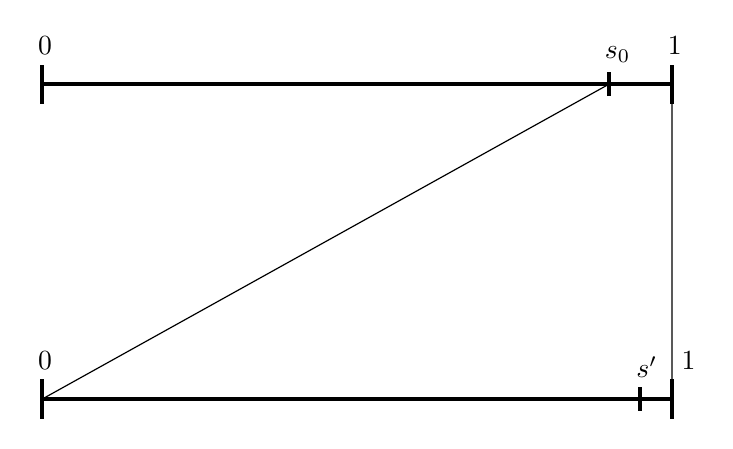
\begin{tikzpicture}
\draw [line width=0.5mm] (0, 0) -- (8, 0)
      (0, -0.25) -- (0, 0.25)
      (8, -0.25) -- (8, 0.25)
      (7.2, -0.15) -- (7.2, 0.15)
      [line width=0.5mm] (0, -4) -- (8, -4)
      (0, -4.25) -- (0, -3.75)
      (8, -4.25) -- (8, -3.75)
      (7.6, -4.15) -- (7.6, -3.85);
      
      \draw [line width=0.15mm] (7.2, 0) -- (0, -4)
      [line width=0.15mm] (8, 0) -- (8, -4)
      ;
      \draw (-0.175, 0.25) node[anchor=south west] {0};
      \draw (8-0.175, 0.25) node[anchor=south west] {1};
      \draw (7.2-0.175, 0.15) node[anchor=south west] {$s_0$};

      \draw (-0.175, 0.25-4) node[anchor=south west] {0};
      \draw (8, 0.25-4) node[anchor=south west] {1};
      \draw (7.6-0.175, 0.15-4) node[anchor=south west] {$s'$};

% \draw (0.6, 2) node[anchor=south west] {Bus $i$};
% \draw (6.6, 2) node[anchor=south west] {Bus $j$};
% \draw (3.8, 1.6) node[anchor=south west] {$Y$};
% \draw (1, 1) node[anchor=north west] {$U_i$};
% \draw (7, 1) node[anchor=north east] {$U_j$};
% \draw (-0.4, 0) node[anchor=north east] {$S_i$};
% \draw (8.4, 0) node[anchor=north west] {$S_j$};
    \end{tikzpicture}
    \caption{Ampliació que realitza el P-W}
    \label{fig:PWzoom}
    \end{center}
    \end{figure}

La idea al darrere de la transformació conforme resideix en avaluar sèries en les quals els aproximants de Padé convergeixin. Si en el cas exemplificat això passa per $s'=$ 0,95, amb l'Equació \ref{eq.pw1} es dedueix que $s=$ 0,995. D'aquest mode el P-W tracta d'apropar-se a $s=1$ per mitjà de solucions parcials.

El P-W està pensat per dur a terme diverses ampliacions d'aquesta mena, de fet, tantes com sigui necessari. Cada un d'aquests passos s'anomenarà graó. Primer es dedueixen les expressions per un graó i llavors es generalitza. Se segueix la formulació original. L'adaptació del P-W a la formulació pròpia implica retardar a cada graó algunes expressions, i en aquest cas, el mètode es veu perjudicat.

\section{Primer graó}
Es desenvolupen les equacions del P-W a partir de la formulació original, ja que en comptar amb $V[0]=1$ i $Q[0]=0$ les expressions se simplifiquen, i sobretot, permeten plantejar un algoritme escalable. 

També es tracta de replicar un sistema d'equacions com el de l'algoritme original: una matriu constant a tots els passos i que només es factoritza una vegada per cada graó, un vector amb les incògnites d'ordre $c$ i un vector calculable amb coeficients d'ordre $c-1$ o inferior.

D'entrada es treballa amb expressions compactes, és a dir, que el bus oscil·lant forma part del mateix vector que els busos PQ i PV. No es tracta per separat. La fragmentació de la matriu d'admitàncies en $Y^{(a)}$ i $Y^{(b)}$ es deixa per més endavant. No obstant això, de cara a la implementació del mètode resulta un aspecte clau.

\subsection{Busos PQ}
El desenvolupament per als busos PQ comença amb el balanç d'intensitats a un bus $i$. Els factors de la dreta de la igualtat es multipliquen per $s$, el que implica que el seu càlcul es retardi un pas:
\begin{equation}
    \sum_{j}Y_{ij}V_j(s)=-sY_{sh,i}V_i(s)+s\frac{S^*_i}{V^*_i(s^*)}\ .
        \label{eq:P1}
\end{equation}
A partir d'ara, per comoditat les expressions de l'estil $X^*(s^*)$ es converteixen a $X^*(s)$ perquè $s$ ha de ser forçosament real. El mètode parteix de $s=0$ i avança cap a $s=1$ sempre al llarg de l'eix real (Trias, 2018). Aleshores es realitza la transformació conforme de la variable $s$, tal com es dedueix de l'Equació \ref{eq.pw1}. També s'introdueix una nova sèrie de tensió per cada bus incògnita:
\begin{equation}
    \begin{cases}
    \begin{split}
        s&=s_0+s'(1-s_0),\\
        V_i(s)&=V'_i(s')V_i(s_0)\ ,
    \end{split}
\end{cases}
        \label{eq:P2}
\end{equation}
on:

$V'_i(s')$: nova sèrie de tensió a calcular.
\vs
$V_i(s_0)$: sèrie de tensió inicial avaluada a $s_0$. És una solució parcial.

De manera que la combinació de les Equacions \ref{eq:P1} i \ref{eq:P2} dóna peu a:
\begin{equation}
    \sum_{j}Y_{ij}V'_j(s')V_j(s_0)=-(s_0+s'(1-s_0))Y_{sh,i}V'_i(s)V_i(s_0)+(s_0+s'(1-s_0))\frac{S^*_i}{V'^{*}_i(s')V^*_i(s_0)}\ .
        \label{eq:P3}
\end{equation}
Cada costat de l'equació es multiplica per $V^*_i(s_0)$ per tal fer-lo desaparèixer del denominador de l'últim sumand:
\begin{equation}
    \sum_{j}Y_{ij}V'_j(s')V_j(s_0)V^*_i(s_0)=-(s_0+s'(1-s_0))Y_{sh,i}V'_i(s)|V_i(s_0)|^2+(s_0+s'(1-s_0))\frac{S^*_i}{V'^{*}_i(s')}\ .
        \label{eq:P4}
\end{equation}
Es reordenen termes per veure per què el penúltim terme és conflictiu fins a cert punt:
\begin{equation}
    \begin{split}
    \sum_{j}Y_{ij}V'_j(s')V_j(s_0)V^*_i(s_0)+s_0Y_{sh,i}V'_i(s)|V_i(s_0)|^2&=-s'(1-s_0)Y_{sh,i}V'_i(s)|V_i(s_0)|^2\\
    &+s_0\frac{S^*_i}{V'^{*}_i(s')}+s'(1-s_0)\frac{S^*_i}{V'^{*}_i(s')}\ .
    \end{split}
        \label{eq:P5}
\end{equation}
Tots els sumands de la dreta de l'igual, excepte un, es troben multiplicats per $s'$; així el seu ús queda retardat i no intervenen els coeficients del mateix ordre dels de l'esquerra de l'igual. En el penúltim terme això no passa, de forma que $V'^{*}_i(s')$ es troba al denominador, el que complica la resolució. Per fer-li front es treballa amb:
\begin{equation}
    s_0\frac{S^*_i}{V'^{*}_i(s')} = s_0S^*_iV'_i(s')+s_0S^*_i\biggl(\frac{1}{V'^{*}_i(s')}-V'_i(s')\biggr)\ .
        \label{eq:P6}
\end{equation}
L'avantatge d'introduir aquesta aparent complicació es manifesta en tenir en compte que els primers termes de la sèrie $V'_i(s')$ també han de valdre 1, igual que es buscava per $V_i(s)$. Així, quan es calculen els primers coeficients de les incògnites, l'Equació \ref{eq:P6} esdevé:
\begin{equation}
    s_0\frac{S^*_i}{V'^{*}_i(s')} = s_0S^*_iV'_i(s')\ .
        \label{eq:P6x}
\end{equation}
La sèrie $V'_i(s')$ es troba al numerador. Això permet progressar amb la construcció del sistema lineal d'equacions. Així, amb aquesta modificació l'Equació \ref{eq:P5} passa a ser:
% \begin{equation}
%     \begin{split}
%     \sum_{j}Y_{ij}V'_j(s')V_j(s_0)V^*_i(s_0)&+s_0Y_{sh,i}V'_i(s)|V_i(s_0)|^2-s_0S^*_iV'_i(s')=\\
%     &-s'(1-s_0)Y_{sh,i}V'_i(s)|V_i(s_0)|^2+s'(1-s_0)\frac{S^*_i}{V'^{*}_i(s')}\\
%     &+s_0S^*_i\biggl(\frac{1}{V'^{*}_i(s')}-V'_i(s')\biggr)\ .
%     \end{split}
%         \label{eq:P7}
% \end{equation}
\begin{equation}
    \begin{split}
    \sum_{j}&Y_{ij}V'_j(s')V_j(s_0)V^*_i(s_0)+s_0Y_{sh,i}V'_i(s)|V_i(s_0)|^2-s_0S^*_iV'_i(s')=\\
    &-s'(1-s_0)Y_{sh,i}V'_i(s)|V_i(s_0)|^2+s'(1-s_0)\frac{S^*_i}{V'^{*}_i(s')}
    +s_0S^*_i\biggl(\frac{1}{V'^{*}_i(s')}-V'_i(s')\biggr)\ .
    \end{split}
        \label{eq:P7}
\end{equation}
En aquest punt només falta desenvolupar el darrer terme. S'assumeix que $V_i[0]=1$ de manera que en forma de coeficients, per $c\geq1$:
\begin{equation}
    s_0S^*_i\biggl(\frac{1}{V'^*_i(s^*)}-V'_i(s')\biggr)\equiv s_0S^*_i\biggl(-2V'^{(re)}_i[c]-\sum_{k=1}^{c-1}X'_i[k]V'^{*}_i[c-k]\biggr)\ ,
        \label{eq:P8}
\end{equation}
on $X'_i(s')$ és la inversa de $V'^*_i(s')$. Amb tot això l'equació definitiva per als busos PQ en el primer graó és:
% \begin{equation}
%     \begin{split}
%     \sum_{j}Y_{ij}V'_j[c]V_j(s_0)V^*_i(s_0)&+s_0Y_{sh,i}V'_i[c]|V_i(s_0)|^2-s_0S^*_iV'_i[c]\\ +2s_0S^*_iV'^{(re)}_i[c]=
%     &-(1-s_0)Y_{sh,i}V'_i[c-1]|V_i(s_0)|^2+(1-s_0)S^*_iX'_i[c-1]\\
%     &+s_0S^*_i\biggl(-\sum_{k=1}^{c-1}X'_i[k]V'^{*}_i[c-k]\biggr)\ ,
%     \end{split}
%         \label{eq:P9}
% \end{equation}
\begin{equation}
    \begin{split}
    \sum_{j}&Y_{ij}V'_j[c]V_j(s_0)V^*_i(s_0)+s_0Y_{sh,i}V'_i[c]|V_i(s_0)|^2-s_0S^*_iV'_i[c] +2s_0S^*_iV'^{(re)}_i[c]=\\
    &-(1-s_0)Y_{sh,i}V'_i[c-1]|V_i(s_0)|^2+(1-s_0)S^*_iX'_i[c-1]
    +s_0S^*_i\biggl(-\sum_{k=1}^{c-1}X'_i[k]V'^{*}_i[c-k]\biggr)\ ,
    \end{split}
        \label{eq:P9}
\end{equation}
que s'utilitza per a $c\geq 1$. Tal com en un principi interessava, a l'esquerra hi ha les incògnites d'ordre $c$ i a la dreta termes que depenen de l'ordre $c-1$ o inferior. 

\subsection{Busos PV}
La deducció de les equacions per als busos PV inicia també amb el sumatori d'intensitats en un bus $i$. La diferència amb els busos PQ està en el fet que la incògnita $Q_i(s)$ no es troba retardada en el càlcul:
\begin{equation}
    \sum_j Y_{ij}V_j(s)=-sY_{sh,i}V_i(s)+s\frac{P_i}{V^*_i(s)}-j\frac{Q_i(s)}{V^*_i(s)}\ .
        \label{eq:P10}
\end{equation}
En aquest tipus de bus s'introdueixen les tres expressions següents:
\begin{equation}
    \begin{cases}
    \begin{split}
    s&=s_0+s'(1-s_0)\ ,\\
    V_i(s)&=V'_i(s')V_i(s_0)\ ,\\
    Q_i(s)&=Q_i(s_0)+Q'_i(s')\ ,
    \end{split}
\end{cases}
        \label{eq:P11}
\end{equation}
on les dues primeres són idèntiques que les utilitzades per als busos PQ. En aquest cas es crea una nova sèrie de potència reactiva $Q'_i(s')$ per cada un dels busos PV, que se sumen a la solució parcial de reactiva $Q_i(s_0)$. 

Aleshores s'introdueixen les expressions de l'Equació \ref{eq:P11} a l'Equació \ref{eq:P10}. Amb unes quantes manipulacions directes en resulta:
% \begin{equation}
%     \begin{split}
%     \sum_j Y_{ij}V_j(s_0)V^*_i(s_0)V'_j(s')&+(s_0+s'(1-s_0))Y_{sh,i}|V_i(s_0)|^2V'_i(s')=s_0\frac{P_i}{V'^{*}_i(s')}\\
%     &+s'(1-s_0)\frac{P_i}{V'^{*}_i(s')} -j\frac{Q_i(s_0)}{V'^{*}_i(s')}-j\frac{Q'_i(s')}{V'^{*}_i(s')}=\Psi\ , 
% \end{split}
%         \label{eq:P12}
% \end{equation}
\begin{equation}
    \begin{split}
    \sum_j &Y_{ij}V_j(s_0)V^*_i(s_0)V'_j(s')+(s_0+s'(1-s_0))Y_{sh,i}|V_i(s_0)|^2V'_i(s')=\\
    &s_0\frac{P_i}{V'^{*}_i(s')}
    +s'(1-s_0)\frac{P_i}{V'^{*}_i(s')} -j\frac{Q_i(s_0)}{V'^{*}_i(s')}-j\frac{Q'_i(s')}{V'^{*}_i(s')}=\Psi\ , 
\end{split}
        \label{eq:P12}
\end{equation}
on $\Psi$ equival al costat de la dreta de la igualtat, que s'ha de desenvolupar. 

Tots aquells sumands que no depenen de $s'$ en el numerador passen per una transformació com la dels busos PQ:
\begin{equation}
    \Psi = s'(1-s_0)\frac{P_i}{V'^{*}_i(s')}-j\frac{Q'_i(s')}{V'^{*}_i(s')}+(s_0P_i-jQ_i(s_0))\biggl(\frac{1}{V'^{*}_i(s')}-V'_i(s')\biggr)+(s_0P_i-jQ_i(s_0))V'_i(s')\ .
    \label{eq:P13}
\end{equation} 
Així, els termes que contenen incògnites de l'ordre a calcular es mouen al costat esquerre de l'Equació \ref{eq:P12}, mentre que a la dreta hi apareixen les expressions que s'anul·len a l'hora d'obtenir els primers coeficients.

Tot plegat porta al següent:
% \begin{equation}
%     \begin{split}
%     \sum_j Y_{ij}V_j(s_0)V^*_i(s_0)V'_j(s')&+s_0Y_{sh,i}|V_i(s_0)|^2V'_i(s')-s_0P_iV'_i(s')+jQ_i(s_0)V'_i(s')=\\
%     &-s'(1-s_0)Y_{sh,i}|V_i(s_0)|^2V'_i(s')+s'(1-s_0)\frac{P_i}{V'^{*}_i(s')}\\
%     &+(s_0P_i-jQ_i(s_0))\biggl(\frac{1}{V'^{*}_i(s')}-V'_i(s')\biggr)-j\frac{Q'_i(s')}{V'^{*}_i(s')}\ .   
% \end{split}
%         \label{eq:P14}
% \end{equation}
\begin{equation}
    \begin{split}
    \sum_j &Y_{ij}V_j(s_0)V^*_i(s_0)V'_j(s')+s_0Y_{sh,i}|V_i(s_0)|^2V'_i(s')-s_0P_iV'_i(s')+jQ_i(s_0)V'_i(s')=\\
    &-s'(1-s_0)Y_{sh,i}|V_i(s_0)|^2V'_i(s')+s'(1-s_0)\frac{P_i}{V'^{*}_i(s')}-j\frac{Q'_i(s')}{V'^{*}_i(s')}\\
    &+(s_0P_i-jQ_i(s_0))\biggl(\frac{1}{V'^{*}_i(s')}-V'_i(s')\biggr)\ .   
\end{split}
        \label{eq:P14}
\end{equation}
Ara només manca desfer-se dels denominadors on apareix la tensió incògnita. Això implica realitzar algunes convolucions, amb la qual cosa en forma de termes s'arriba a:
% \begin{equation}
%     \begin{split}
%     \sum_j Y_{ij}V_j(s_0)V^*_i(s_0)V'_j[c]&+s_0Y_{sh,i}|V_i(s_0)|^2V'_i[c]-s_0P_iV'_i[c]+jQ_i(s_0)V'_i[c]\\
%     &+2(s_0P_i-jQ_i(s_0))V'^{(re)}_i[c]+jQ'_i[c]=-(1-s_0)Y_{sh,i}|V_i(s_0)|^2V'_i[c-1]\\
%     &+(1-s_0)P_iX'_i[c-1]-j\sum_{k=1}^{c-1}Q'_i[k]X'_i[c-k]\\
%     &+(s_0P_i-jQ_i(s_0))\biggl(-\sum_{k=1}^{c-1}X'_i[k]V'^{*}_i[c-k]\biggr)\ . 
% \end{split}
%         \label{eq:P15}
% \end{equation}
\begin{equation}
    \begin{split}
    \sum_j &Y_{ij}V_j(s_0)V^*_i(s_0)V'_j[c]+s_0Y_{sh,i}|V_i(s_0)|^2V'_i[c]-s_0P_iV'_i[c]+jQ_i(s_0)V'_i[c]\\
    &+2(s_0P_i-jQ_i(s_0))V'^{(re)}_i[c]+jQ'_i[c]=
    -(1-s_0)Y_{sh,i}|V_i(s_0)|^2V'_i[c-1]\\
    &+(1-s_0)P_iX'_i[c-1]-j\sum_{k=1}^{c-1}Q'_i[k]X'_i[c-k]
    +(s_0P_i-jQ_i(s_0))\biggl(-\sum_{k=1}^{c-1}X'_i[k]V'^{*}_i[c-k]\biggr)\ . 
\end{split}
        \label{eq:P15}
\end{equation}
S'observa que l'Equació \ref{eq:P15}, que és la pròpia dels busos PV des del punt de vista de balanç d'intensitats, s'assimila molt a la dels PQ (Equació \ref{eq:P9}). 

Com que les incògnites d'ordre $c$ depenen de termes d'ordre $c-1$ o inferior, quan $c=0$ la dreta de la igualtat és nul·la. Això permet que les noves tensions siguin unitàries i que el primer terme de potència reactiva esdevingui 0.

Cal deixar clar que a l'Equació \ref{eq:P9} el terme $2s_0S^{*}_iV'^{(re)}_i[c]$ és inexistent per $c=0$. Succeeix el mateix per l'expressió $2(s_0P_i-jQ_i(s_0))V'^{(re)}_i[c]$ de l'Equació \ref{eq:P15}, mentre que $jQ'_i[0]$ és nul. D'aquesta manera la inicialització és idèntica a la de la formulació original del MIH bàsic.  

Pel que fa als mòduls de voltatge dels busos PV, en un principi es plantejava:
\begin{equation}
V_i(s)V^*_i(s^*)=1+s(W_i-1)\ .
        \label{eq:P15x1}
\end{equation}
Si en aquesta equació se li apliquen les transformacions, queda:
\begin{equation}
    V_i(s_0)V'_i(s')V^*_i(s_0)V'^{*}_i(s')=1+(s_0+s'(1-s_0))(W_i-1)\ ,
            \label{eq:P15x2}
    \end{equation}
que pot no ser consistent amb $V'_i[0]=1$. 

Per això, és necessari convertir-la en:
\begin{equation}
    |V_i(s_0)|^2V'_i(s')V'^{*}_i(s')=|V_i(s_0)|^2+s'(W_i-|V_i(s_0)|^2)\ .
            \label{eq:P15x3}
    \end{equation}
D'aquesta manera es garanteix que l'Equació \ref{eq:P15x3} mantingui coherència amb $V'_i[0]=1$. Resulta necessari assumir que d'entrada $|V_i(s_0)| \neq 1$. L'Equació \ref{eq:P15x3} es pot simplificar en:
\begin{equation}
    V'_i(s')V'^{*}_i(s')=1+s'\biggl(\frac{W_i}{|V_i(s_0)|^2}-1\biggr)\ .
            \label{eq:P15x4}
    \end{equation}
El plantejament de les equacions com a tal s'acaba aquí. Tot i això, convé compactar més les expressions per facilitar la comprensió del mètode i afavorir la seva programació. Se simplifiquen les expressions per mitjà de canvis de variable. A més, a la implementació se separa en part real i imaginària i el bus oscil·lant es tracta per separat. 

\subsection{Compactació}
Igual que a la formulació original, es considera que només hi ha un bus oscil·lant en tot el sistema. Aquest bus també passa per la transformació de tensions:
\begin{equation}
    V_w(s)=V'_w(s')V_w(s_0)\ .
    \label{eq:C1}
\end{equation}
Altre cop es necessita que el primer coeficient de la nova sèrie $V'_w(s')$ valgui 1. De no ser així, el desenvolupament anterior queda invalidat. De manera que en aïllar $V'_w(s')$ i en tenir present que $s=s_0+s'(1-s_0)$, la nova tensió del bus oscil·lant s'incrusta així:
\begin{equation}
    V'_w(s')=1+s'\frac{(1-s_0)(V_w-1)}{1+s_0(V_w-1)}\ ,
    \label{eq:C2}
\end{equation}
on per descomptat es compleix que $V'_w[0]$ valgui 1. 

D'acord amb Trias (2018) es crea el paràmetre $\Gamma_i$ per simplificar les expressions:
\begin{equation}
    \begin{cases}
    \begin{split}
    \Gamma_{i\in PQ}&=s_0S^{*}_i\ ,\\
    \Gamma_{i\in PV}&=s_0P_i-jQ_i(s_0)\ .
    \end{split}
\end{cases}
    \label{eq:C4}
\end{equation}
Quant a la matriu d'admitàncies, tal com s'exposa a la formulació original, està composta per $Y^{(b)}$ i per $Y^{(a)}$. De fet, a les Equacions \ref{eq:P9} i \ref{eq:P15} la matriu $Y$ queda multiplicada per les solucions parcials. Per tant, s'introdueix el canvi de variable:
\begin{equation}
    \begin{cases}
    \begin{split}
        \widehat{Y}^{(a)}_{ij} &= {Y}^{(a)}_{ij}V_j(s_0)V^*_i(s_0)\ ,\\
        \widehat{Y}^{(b)}_{ij} &= {Y}^{(b)}_{ij}V_j(s_0)V^*_i(s_0)\ ,\\
    \end{split}
\end{cases}
    \label{eq:sy1}
\end{equation}
on ara s'estima que $\widehat{Y}^{(a)}$ és asimètrica i les seves files no sumen 0 però no hi ha motius per assegurar res d'això no passi per a $\widehat{Y}^{(b)}$. 

Per lluitar contra això s'ha de tenir present que si es desitja que tots els primers coeficients de tensió siguin 1, tant de l'Equació \ref{eq:P9} com de l'Equació \ref{eq:P15} es dedueix:
\begin{equation}
    \sum_{j}\widehat{Y}^{(b)}_{ij}*1+s_0Y_{sh,i}*1*|V_i(s_0)|^2-\Gamma_i*1=0\ ,
    \label{eq:C6}
\end{equation}
és a dir, que permet conèixer quant val la suma de qualsevol fila:
\begin{equation}
    \sum_{j}\widehat{Y}^{(b)}_{ij}=-s_0Y_{sh,i}|V_i(s_0)|^2+\Gamma_i\ .
    \label{eq:C7}
\end{equation}
Així, s'ha de restar aquesta expressió a algun terme de la fila $i$. Llavors, la suma dels elements d'una fila serà nul·la, tal com interessa per fixar que $V'[0]=1$. S'escull modificar els elements que conformen la diagonal:
\begin{equation}
    \begin{cases}
    \begin{split}
        \widetilde{Y}^{(b)}_{ij}&= \widehat{Y}^{(b)}_{ij}\text{\hspace{77pt} si }j\neq i\ ,\\
        \widetilde{Y}^{(b)}_{ij}&= \widehat{Y}^{(b)}_{ij}-\sum_{j}\widehat{Y}^{(b)}_{ij}\text{\hspace{31.5pt} si }j=i\ .\\
    \end{split}
\end{cases}
    \label{eq:C8}
\end{equation}
El procediment a seguir tant si $i$ es refereix a un bus PQ com a un bus PV és idèntic. L'únic que canvia és el terme $\Gamma_i$, que segueix l'Equació \ref{eq:C4}.

Tanmateix, falta tenir en compte que en la formulació original la matriu d'admitàncies resultava ser $Y=Y^{(b)}+sY^{(a)}$. Com que $s$ pateix la transformació de l'Equació \ref{eq:P2}, queda:
\begin{equation}
    Y=Y^{(b)}+s_0Y^{(a)}+s'(1-s_0)Y^{(a)}\ .
    \label{eq:sy5}
\end{equation}
Es nota que per un costat els dos primers sumands no depenen de $s'$, però l'últim sí. 

Així, cal tenir en compte aquestes modificacions, pel que les matrius definitives s'actualitzen amb les assignacions següents:
\begin{equation}
    \begin{cases}
    \begin{split}
    \widetilde{Y}^{(b)}&:= \widetilde{Y}^{(b)}+s_0\widehat{Y}^{(a)}\ ,\\
    \widehat{Y}^{(a)}&:= (1-s_0)\widehat{Y}^{(a)}\ ,
    \end{split}
\end{cases}
    \label{eq:sy6}
\end{equation}
on finalment ara sí que totes les files de la matriu $\widetilde{Y}^{(b)}$ sumen 0. 

Es nota que igual que en el MIH bàsic, les matrius del tipus $Y^{(a)}$ estan retardades. En conseqüència, no influeixen a l'hora de calcular els primers termes, i com que en el cas de $Y^{(b)}$ les files sumen 0, s'aconsegueix l'estat de referència. Per tant, en el Padé-Weierstrass és necessari que la matriu $\widehat{Y}^{(a)}$ es trobi retardada en el càlcul.

\subsection{Algoritme}
En aquest punt s'han adaptat les matrius d'admitàncies segons convenia i es disposa de les Equacions \ref{eq:P9}, \ref{eq:P15} i \ref{eq:P15x4}. Convé plantejar de forma més explícita els passos en què consisteix l'algoritme resolutiu, així com esbrinar quines expressions intervenen en el sistema lineal d'equacions. 

Per als busos PQ la dreta de l'igual de l'Equació \ref{eq:P9}, que s'anomena $\Psi$, esdevé:
\begin{equation}
    \begin{split}
    \Psi_{i\in PQ}=&-\sum_{j}\widehat{Y}^{(a)}_{ij}V'_j[c-1]
    -(1-s_0)Y_{sh,i}V'_i[c-1]|V_i(s_0)|^2+(1-s_0)S^*_iX'_i[c-1]\\
    &+s_0S^*_i\biggl(-\sum_{k=1}^{c-1}X'_i[k]V'^{*}_i[c-k]\biggr)\ .
    \end{split}
        \label{eq:C10}
\end{equation}
L'efecte d'afegir la matriu $\widehat{Y}^{(a)}$ ve a ser el mateix que afegir la injecció que provoquen els elements com transformadors de relació variable, encara que en el P-W queda multiplicada per $1-s_0$. Això fa que les seves entrades no tinguin gaire pes. De fet, a cada graó s'empetiteix més.

En el codi, els elements del tipus $\widehat{Y}^{(a)}_{ij}$ es divideixen en aquells on els busos $j$ són PQ i PV i per altre costat, en els elements que prenen l'índex del bus oscil·lant. El bus oscil·lant només intervé en els primers ordres, tal com posa de manifest l'Equació \ref{eq:C2}. No obstant això, aquesta distinció no s'ha tingut en compte en el desenvolupament per no complicar més les expressions.

En els busos PV la dreta de l'igual de l'Equació \ref{eq:P15} es converteix en:
% \begin{equation}
%     \begin{split}
%     \Psi_{i\in PV}=&-\sum_{j}\widehat{Y}^{(a)}_{ij}V'_j[c-1]
%     -(1-s_0)Y_{sh,i}|V_i(s_0)|^2V'_i[c-1]\\
%     &+(1-s_0)P_iX'_i[c-1]-j\sum_{k=1}^{c-1}Q'_i[k]X'_i[c-k]\\
%     &+(s_0P_i-jQ_i(s_0))\biggl(-\sum_{k=1}^{c-1}X'_i[k]V'^{*}_i[c-k]\biggr)\ . 
%     \end{split}
%         \label{eq:C11}
% \end{equation}
\begin{equation}
    \begin{split}
    \Psi_{i\in PV}=&-\sum_{j}\widehat{Y}^{(a)}_{ij}V'_j[c-1]
    -(1-s_0)Y_{sh,i}|V_i(s_0)|^2V'_i[c-1]\\
    &+(1-s_0)P_iX'_i[c-1]-j\sum_{k=1}^{c-1}Q'_i[k]X'_i[c-k]
    +(s_0P_i-jQ_i(s_0))\biggl(-\sum_{k=1}^{c-1}X'_i[k]V'^{*}_i[c-k]\biggr)\ . 
    \end{split}
        \label{eq:C11}
\end{equation}
Anàlogament el bus oscil·lant també es pot separar explícitament en dues parts. La matriu $\widetilde{Y}^{(b)}$ encara conté la connexió amb el bus oscil·lant, que no és una incògnita. Per això cal fragmentar-la. 

En aquest aspecte el bus oscil·lant només apareix a l'ordre $c=1$ perquè $\widetilde{Y}^{(b)}$ no està retardada i $c=0$ es correspon a l'estat de referència on no se soluciona directament cap sistema d'equacions. La matriu $\widetilde{Y}^{(b)}$ reduïda, que no compta amb elements que representen la connexió amb el bus oscil·lant, es denota per $\widetilde{Y}^{(b,red)}$. 

L'Equació \ref{eq:C10} esdevé:
\begin{equation}
    \begin{split}
    \Psi_{i\in PQ}=&-\widetilde{Y}^{(b)}_{iw}V'_w[c]-\sum_{j}\widehat{Y}^{(a)}_{ij}V'_j[c-1]
    -(1-s_0)Y_{sh,i}V'_i[c-1]|V_i(s_0)|^2\\
    &+(1-s_0)S^*_iX'_i[c-1]+s_0S^*_i\biggl(-\sum_{k=1}^{c-1}X'_i[k]V'^{*}_i[c-k]\biggr)\ ,
    \end{split}
        \label{eq:C12}
\end{equation}
on $\widetilde{Y}^{(b)}_{iw}$ és l'element extret de la $\widetilde{Y}^{(b)}$ total que enllaça amb l'oscil·lant. 

L'Equació \ref{eq:C11} passa a ser:
% \begin{equation}
%     \begin{split}
%     \Psi_{i\in PV}=&-\widetilde{Y}^{(b)}_{iw}V'_w[c]
%     -\sum_{j}\widehat{Y}^{(a)}_{ij}V'_j[c-1]
%     -(1-s_0)Y_{sh,i}|V_i(s_0)|^2V'_i[c-1]\\
%     &+(1-s_0)P_iX'_i[c-1]-j\sum_{k=1}^{c-1}Q'_i[k]X'_i[c-k]\\
%     &+(s_0P_i-jQ_i(s_0))\biggl(-\sum_{k=1}^{c-1}X'_i[k]V'^{*}_i[c-k]\biggr)\ .
%     \end{split}
%         \label{eq:C13}
% \end{equation}
\begin{equation}
    \begin{split}
    \Psi_{i\in PV}=&-\widetilde{Y}^{(b)}_{iw}V'_w[c]
    -\sum_{j}\widehat{Y}^{(a)}_{ij}V'_j[c-1]
    -(1-s_0)Y_{sh,i}|V_i(s_0)|^2V'_i[c-1]\\
    &+(1-s_0)P_iX'_i[c-1]-j\sum_{k=1}^{c-1}Q'_i[k]X'_i[c-k]
    +(s_0P_i-jQ_i(s_0))\biggl(-\sum_{k=1}^{c-1}X'_i[k]V'^{*}_i[c-k]\biggr)\ .
    \end{split}
        \label{eq:C13}
\end{equation}
Per a la implementació es calcula la part real i la part imaginària de $\Psi_{i}$, tal com es fa en el MIH bàsic.

Finalment, s'ha de refer l'expressió de l'esquerra de la igualtat, que s'anomena $\Theta$, per determinar també els elements de la matriu del sistema. 
Segons Trias (2018), la seva estructura i dispersió es conserva respecte al MIH original. Les seves entrades canvien però són les mateixes al llarg de tots els passos d'aquell graó del P-W. Així doncs, la matriu només s'ha de factoritzar una vegada per graó.

Per als busos PQ es recupera l'Equació \ref{eq:P9}, s'apliquen els canvis anteriorment esmentats i se la converteix en: 
\begin{equation}
    \Theta_{i\in PQ}=\sum_{j}\widetilde{Y}^{(b,red)}_{ij}V'_j[c]+2\Gamma_iV'^{(re)}_i[c]\ .
        \label{eq:C14}
\end{equation}
Aquesta darrera equació és vàlida a condició que $c\geq 1$, és clar. 

Per als busos PV s'arriba a una expressió molt similar amb la diferència que hi ha la incògnita de potència reactiva:
\begin{equation}
    \Theta_{i\in PV}=\sum_{j}\widetilde{Y}^{(b,red)}_{ij}V'_j[c]+2\Gamma_iV'^{(re)}_i[c]+jQ'_i[c]\ .
        \label{eq:C15}
\end{equation}
Tant els termes de l'Equació \ref{eq:C14} com els de l'Equació \ref{eq:C15} es fragmenten també en part real i imaginària. 

La matriu del sistema en forma de blocs és:
\begin{equation}
    R = 
    \begin{pmatrix}
        G+2\Gamma^{(re)} & -B & 0 \\
        B+2\Gamma^{(im)} & G &  1 \\
        \Upsilon & 0 & 0 
    \end{pmatrix}L\ ,
    \label{eq:MATPW}
\end{equation}
on:

$\Gamma^{(re)}$: matriu diagonal formada per les parts reals dels paràmetres $\Gamma_i$. 
\vs
$\Gamma^{(im)}$: matriu diagonal formada per les parts imaginàries dels paràmetres $\Gamma_i$. 
\vs
$G$: part real de la matriu $\widetilde{Y}^{(b,red)}$.
\vs
$B$: part imaginària de la matriu $\widetilde{Y}^{(b,red)}$.

La resta de matrius són idèntiques a les de l'Equació \ref{eq:quadri2MIH2}. Els vectors $R$ i $L$ segueixen la mateixa ordenació, encara que ara $R$ és definit per $\Psi$ i $L$ inclou les incògnites $V'^{(re)}$, $V'^{(im)}$ i $Q'$. 

A tall d'exemple la Figura \ref{fig:PWstep1} compara com evoluciona la grandària dels termes amb el MIH bàsic i amb el primer graó del P-W per al bus 1 de la xarxa de test Nord Pool. 

\begin{figure}[!htb] \footnotesize
    \begin{center}
    \begin{tikzpicture}
    \begin{axis}[
        /pgf/number format/.cd, use comma, 1000 sep={.}, ylabel={$\log |V[i]|$},xlabel={Ordre del terme, $i$},domain=0:5, ylabel style={rotate=-90},legend style={at={(1,0)},anchor=south west},width=9cm,height=7.5cm,scatter/classes={%
        a={mark=x,mark size=2pt,draw=black}, b={mark=*,mark size=2pt,draw=black}, c={mark=o,mark size=2pt,draw=black}%
        ,d={mark=diamond,mark size=2pt,draw=black}, e={mark=+,mark size=2pt,draw=black}, f={mark=triangle,mark size=2pt,draw=black}}]]
    \addplot[scatter,scatter src=explicit symbolic]%
        table[x = x, y = y, meta = label, col sep=semicolon] {Inputs/sensePW.csv};
    \addplot[scatter,scatter src=explicit symbolic]%
        table[x = x, y = y, meta = label, col sep=semicolon] {Inputs/sensePW2.csv};
        \legend{$|V_{1}[i]|$, ,$|V'_{1}[i]|$} %tocar
        \end{axis}
    \end{tikzpicture}
    \caption{Evolució de les sèries de la tensió del bus 1 del Nord Pool per $s_0=$\ 0,5}
    \label{fig:PWstep1}
    \end{center}
    \end{figure}

S'observa com els termes que conformen la tensió $V'_{1}$ s'empetiteixen més ràpidament. Així, aquesta nova sèrie millora pel que fa a la convergència. La solució final que proporciona el P-W de només un graó fa ús de les Equacions \ref{eq:P2} i \ref{eq:P11}, on avalua les noves sèries a $s'=1$ i d'aquesta manera obté les incògnites definitives $V(s)$ i $Q(s)$. 

\section{Generalització}
A la Figura \ref{fig:PWstep1} la convergència dels termes s'accelera, tot i que no necessàriament l'error esdevé prou satisfactori. L'algoritme del P-W consisteix a trobar tantes sèries noves com faci falta per minimitzar l'error. Per això cal generalitzar el P-W per un graó qualsevol. De fet, com més mal condicionat es troba un sistema, habitualment més graons es necessiten.

Es comença amb les expressions per a dos graons, on la variable $s$ obeeix:
\begin{equation}
    s=s_0+s'(1-s_0)=s_0+s'_0(1-s_0)+s''(1-s_0)(1-s'_0)\ .
    \label{eq:pw2_s}
\end{equation}
En aquest cas, $s''$ intervé com a variable; $s_0$ i $s'_0$ són dades. En expandir l'Equació \ref{eq:pw2_s}, es nota que tot plegat es pot compactar de forma general per mitjà de:
\begin{equation}
    s = \gamma^{(r)} + s^{(r)}(1-\gamma^{(r)})\ ,
    \label{eq:pw2_gamm}
\end{equation}
on:

$r$: indicador del graó actual. Al segon graó, $r=2$.
\vs
$\gamma^{(r)}$: variable que agrupa els termes que no multipliquen $s^{(r)}$. Per a dos graons val $s_0+s'_0-s_0s'_0$. S'ha d'actualitzar a cada graó.
\vs
$s^{(r)}$: variable complexa del graó actual. Quan es treballa amb dos graons, 
$s^{(r)}$ simbolitza $s''$.

\subsection{Busos PQ}
Es procedeix a observar el patró que segueix l'equació que obeeixen els busos PQ al segon graó, encara amb la notació antiga:
\begin{equation}
    \begin{split}
        \sum_j&Y_{ij}V_j(s_0)V^*_i(s_0)V'_j(s'_0)V''_j(s'')+s_0|V_i(s_0)|^2Y_{sh,i}V'_i(s'_0)V''_i(s'')-s_0S^*_iV'_i(s'_0)V''_i(s'')=\\
        &-(1-s_0)(s'_0+s''(1-s'_0))Y_{sh,i}|V_i(s_0)|^2V'_i(s'_0)V''_i(s'')\\
        &+(1-s_0)(s'_0+s''(1-s'_0))\frac{S^*_i}{V'^*_i(s'_0)V''^*_i(s'')}+s_0S^*_i\biggl(\frac{1}{V'^*_i(s'_0)V''^*_i(s'')}-V'_i(s'_0)V''_i(s'')\biggr)\ .
    \end{split}
    \label{eq:pw2_pq1}
\end{equation}
Similar al desenvolupament inicial, es multiplica a banda i banda per $V'^*_i(s'_0)$ per desfer-se d'aquest terme en els denominadors que apareix. S'arregla i s'arriba a:
\begin{equation}
    \begin{split}
        \sum_j&Y_{ij}V_j(s_0)V^*_i(s_0)V'_j(s'_0)V'^*_i(s'_0)V''_j(s'')+s_0|V_i(s_0)|^2|V'_i(s'_0)|^2Y_{sh,i}V''_i(s'')=s_0\frac{S^*_i}{V''^*_i(s'')}\\
        &-(1-s_0)s'_0Y_{sh,i}|V_i(s_0)|^2|V'_i(s'_0)|^2V''_i(s'')+s''(1-s_0)(1-s'_0)\frac{S^*_i}{V''^*_i(s'')}\\
        &-s''(1-s_0)(1-s'_0)Y_{sh,i}|V_i(s_0)|^2|V'_i(s'_0)|^2V''_i(s'')+(1-s_0)s'_0\frac{S^*_i}{V''^*_i(s'')}\ .
    \end{split}
    \label{eq:pw2_pq2}
\end{equation}
Llavors s'identifiquen els termes que porten $V''_i(s'')$ i que no es veuen retardats per tal d'enviar-los a l'esquerra de la igualtat. També es compacta més l'expressió (encara sense fer servir $\gamma^{(r)}$), i en resulta:
\begin{equation}
    \begin{split}
        \sum_j&Y_{ij}V_j(s_0)V^*_i(s_0)V'_j(s'_0)V'^*_i(s'_0)V''_j(s'')+(s_0+s'_0(1-s_0))|V_i(s_0)|^2|V'_i(s'_0)|^2Y_{sh,i}V''_i(s'')=\\
        &-s''(1-s_0)(1-s'_0)Y_{sh,i}|V_i(s_0)|^2|V'_i(s'_0)|^2V''_i(s'')+s''(1-s_0)(1-s'_0)\frac{S^*_i}{V''^*_i(s'')}\\
        &+(s_0+s'_0(1-s_0))S^*_i\biggl(\frac{1}{V''^*_i(s'')}-V''_i(s'')\biggr)+(s_0+s'_0(1-s_0))S^*_iV''_i(s'')\ .\\
    \end{split}
    \label{eq:pw2_pq3}
\end{equation}
Si s'introdueix $\gamma^{(r)}$ l'Equació \ref{eq:pw2_pq3} esdevé:
\begin{equation}
    \begin{split}
        \sum_j&Y_{ij}V_j(s_0)V^*_i(s_0)V'_j(s'_0)V'^*_i(s'_0)V''_j(s'')+\gamma^{(r)}|V_i(s_0)|^2|V'_i(s'_0)|^2Y_{sh,i}V''_i(s'')-\gamma^{(r)} S^*_iV''_i(s'')=\\
        &-s''(1-\gamma^{(r)})Y_{sh,i}|V_i(s_0)|^2|V'_i(s'_0)|^2V''_i(s'')+s''(1-\gamma^{(r)})\frac{S^*_i}{V''^*_i(s'')}\\
        &+\gamma^{(r)} S^*_i\biggl(\frac{1}{V''^*_i(s'')}-V''_i(s'')\biggr)\ .
    \end{split}
    \label{eq:pw2_pq4}
\end{equation}
La implicació de treballar amb $\gamma^{(r)}$ es fa evident. L'expressió final es compacta. A més, $\gamma^{(r)}$ és la mateixa per a qualsevol bus en un graó donat. En afegir la notació al complet:
\begin{equation}
    \begin{split}
   \sum_j&Y_{ij}V^{(r)}_j(s^{(r)})\prod_{k=0}^{r-1}V^{*{(k)}}_i(s^{(k)}_0)V^{{(k)}}_j(s^{(k)}_0)+\gamma^{(r)}Y_{sh,i}V^{(r)}_i(s^{(r)})\prod_{k=0}^{r-1}|V^{(k)}_i(s^{(k)}_0)|^2-\Gamma^{(r)}V^{(r)}_i(s^{(r)})=\\
   &-s^{(r)}(1-\gamma^{(r)})Y_{sh,i}V^{(r)}_i(s^{(r)})\prod_{k=0}^{r-1}|V^{(k)}_i(s^{(k)}_0)|^2+s^{(r)}(1-\gamma^{(r)})\frac{S^*_i}{V^{*(r)}_i(s^{(r)})}\\
        &+\Gamma^{(r)}_i\biggl(\frac{1}{V^{*(r)}_i(s^{(r)})}-V^{(r)}_i(s^{(r)})\biggr)\ ,
    \end{split}
    \label{eq:pw2_pq4x}
\end{equation}
on per les tensions s'ha seguit una notació del mateix estil. Per exemple $V^{(0)}_j(s^{(0)}_0)$ representa $V_j(s_0)$. 

\subsection{Compactació}
De forma similar al raonament per un graó, el P-W generalitzat també guanya en conveniència si les expressions es compacten. En aquest subapartat es detallen algunes definicions útils i necessàries que intervenen en el codi. Les matrius d'admitàncies fragmentades no s'han incorporat a les equacions definitives per als busos PQ i PV perquè en primer lloc es prefereix no entrar encara en més detall en el desenvolupament, i en segon lloc, la seva addició calca la que tenia lloc en el MIH bàsic.

Els nous termes $\Gamma^{(r)}$, que ja s'han usat a l'Equació \ref{eq:pw2_pq4x}, segueixen:
\begin{equation}
    \begin{cases}
    \begin{split}
        \Gamma^{(r)}_{i\in PQ}&=\gamma^{(r)}S^*_i\ .\\
        \Gamma^{(r)}_{i\in PV}&=\gamma^{(r)}P_i-j\sum_{k=0}^{r-1}Q^{(k)}_i(s^{(k)}_0)\ .
    \end{split}
\end{cases}
    \label{eq:Gammar1}
\end{equation}
Pel que fa a les matrius d'admitàncies, també cal fragmentar-les per complir amb l'estat de referència en aquell nou graó. Tal com se'n desprèn de l'Equació \ref{eq:pw2_pq4x}:
\begin{equation}
    \begin{cases}
    \begin{split}
        \widehat{Y}^{(a)}_{ij} &= Y^{(a)}_{ij}\prod_{k=0}^{r-1}V^{*{(k)}}_i(s^{(k)}_0)V^{{(k)}}_j(s^{(k)}_0)\ ,\\
        \widehat{Y}^{(b)}_{ij} &= Y^{(b)}_{ij}\prod_{k=0}^{r-1}V^{*{(k)}}_i(s^{(k)}_0)V^{{(k)}}_j(s^{(k)}_0)\ ,\\
    \end{split}
\end{cases}
    \label{eq:sy1r}
\end{equation}
on igual que amb només un graó s'assumeix que les files de $\widehat{Y}^{(a)}$ i de $\widehat{Y}^{(b)}$ no sumen totes 0, el que és un problema. 

Una d'elles ha d'assegurar l'estat de referència. Es procura solucionar-ho per a $\widehat{Y}^{(b)}$ mitjançant el càlcul de la suma de les seves files:
\begin{equation}
    \sum_{j}\widehat{Y}^{(b)}_{ij}=-\gamma^{(r)}Y_{sh,i}\prod_{k=0}^{r-1}|V^{(k)}_i(s^{(k)}_0)|^2+\Gamma^{(r)}_i\ ,
    \label{eq:C7r}
\end{equation}
on altre cop els primers coeficients de tensió de les sèries valen 1. Igualment es modifiquen els elements de la diagonal:
\begin{equation}
    \begin{cases}
    \begin{split}
        \widetilde{Y}^{(b)}_{ij}&=\widehat{Y}^{(b)}_{ij}\ ,\text{\hspace{77pt} si }j\neq i\ ,\\
        \widetilde{Y}^{(b)}_{ij}&= \widehat{Y}^{(b)}_{ij}-\sum_{j}\widehat{Y}^{(b)}_{ij}\ ,\text{\hspace{31.5pt} si }j=i\ .\\
    \end{split}
\end{cases}
    \label{eq:C8r}
\end{equation}
A causa de la transformació que pateix $s$, les matrius resultants són:
\begin{equation}
    \begin{cases}
    \begin{split}
    \widetilde{Y}^{(b)}&:=\widetilde{Y}^{(b)}+\gamma^{(r)}\widehat{Y}^{(a)}\ ,\\
    \widehat{Y}^{(a)}&:= (1-\gamma^{(r)})\widehat{Y}^{(a)}\ .
    \end{split}
\end{cases}
    \label{eq:sy6r}
\end{equation}
Cada cop $\gamma^{(r)}$ tendeix més cap a l'1, i així, els elements de la matriu $\widehat{Y}^{(a)}$ tenen cada vegada menys pes. Finalment les files de la matriu $\widetilde{Y}^{(b)}$ sumen 0.

\subsection{Busos PV}
En el cas dels busos PV també es desenvolupen les expressions pel segon graó, i llavors es generalitzen. 

Es parteix d'una equació molt similar a la inicial dels PQ, tot i que aquí, per comoditat, ja s'ha eliminat l'element $V'^*_i(s'_0)$ del denominador. En conseqüència, el desenvolupament que segueix comença amb:
\begin{equation}
    \begin{split}
        \sum_j&Y_{ij}V_j(s_0)V^*_i(s_0)V'_j(s'_0)V'^*_i(s'_0)V''_j(s'')+(s_0+s'_0(1-s_0))|V_i(s_0)|^2|V'_i(s'_0)|^2Y_{sh,i}V''_i(s'')=\\
        &-s''(1-s_0)(1-s'_0)Y_{sh,i}|V_i(s_0)|^2|V'_i(s'_0)|^2V''_i(s'')+s'_0(1-s_0)\frac{P_i}{V''^*_i(s'')}\\
        &+ s''(1-s_0)(1-s'_0)\frac{P_i}{V''^*_i(s'')}+\frac{s_0P_i-jQ_i(s_0)-jQ'_i(s'_0)}{V''^*_i(s'')}-\frac{jQ''_i(s'')}{V''^*(s'')}\ .
    \end{split}
    \label{eq:pw2_pv1}
\end{equation}
A continuació s'arregla l'Equació \ref{eq:pw2_pv1} amb l'objectiu de desfer-se de la incògnita del denominador, i queda:
\begin{equation}
    \begin{split}
        \sum_j&Y_{ij}V_j(s_0)V^*_i(s_0)V'_j(s'_0)V'^*_i(s'_0)V''_j(s'')+(s_0+s'_0(1-s_0))|V_i(s_0)|^2|V'_i(s'_0)|^2Y_{sh,i}V''_i(s'')\\
        &-((s_0+s'_0(1-s_0))P_i -j(Q'_i(s'_0)+Q_i(s_0)))V''_i(s'')=\\
        &-s''(1-s_0)(1-s'_0)Y_{sh,i}|V_i(s_0)|^2|V'_i(s'_0)|^2V''_i(s'')
        +s''(1-s_0)(1-s'_0)\frac{P_i}{V''^*_i(s'')}\\
        &+((s_0+s'_0(1-s_0))P_i-j(Q'_i(s'_0)+Q_i(s_0)))\biggl(\frac{1}{V''^*_i(s'')}-V''_i(s'')\biggr)-j\frac{Q''_i(s'')}{V''^*_i(s'')}\ .
    \end{split}
    \label{eq:pw2_pv2}
\end{equation}
La inclusió de $\gamma^{(r)}$ juntament amb la nova notació origina:
\begin{equation}
    \begin{split}
   \sum_j&Y_{ij}V^{(r)}_j(s^{(r)})\prod_{k=0}^{r-1}V^{*{(k)}}_i(s^{(k)}_0)V^{{(k)}}_j(s^{(k)}_0)+\gamma^{(r)}Y_{sh,i}V^{(r)}_i(s^{(r)})\prod_{k=0}^{r-1}|V^{(k)}_i(s^{(k)}_0)|^2-\Gamma^{(r)}V^{(r)}_i(s^{(r)})=\\
   &-s^{(r)}(1-\gamma^{(r)})Y_{sh,i}V^{(r)}_i(s^{(r)})\prod_{k=0}^{r-1}|V^{(k)}_i(s^{(k)}_0)|^2+s^{(r)}(1-\gamma^{(r)})\frac{P_i}{V^{*(r)}_i(s^{(r)})}\\
        &+\Gamma^{(r)}_i\biggl(\frac{1}{V^{*(r)}_i(s^{(r)})}-V^{(r)}_i(s^{(r)})\biggr)-j\frac{Q^{(r)}_i(s^{(r)})}{V^{*(r)}_i(s^{(r)})}\ ,
    \end{split}
    \label{eq:pw2_pv3x}
\end{equation}
on la potència reactiva també segueix la nomenclatura esmentada. 


En últim lloc, quant als mòduls dels busos PV en el segon graó, se sap que obeeixen:
\begin{equation}
    |V_i(s_0)|^2|V'_i(s'_0)|^2V''_i(s'')V''^*_i(s'')=|V_i(s_0)|^2|V'_i(s'_0)|^2+s''(W_i-|V_i(s_0)|^2|V'_i(s'_0)|^2)\ .
    \label{eq:pw2_pv3}
\end{equation}
En lloc de desenvolupar l'equació incrustada amb $s$ del MIH bàsic, es comença amb una nova equació d'aquest estil a cada ordre. Cal que sigui així per tal d'assegurar que el primer terme de tensió de cada sèrie valgui 1. L'Equació \ref{eq:pw2_pv3} es compacta i queda:
\begin{equation}
    V''_i(s'')V''^*_i(s'')=1+s''\biggl(\frac{W_i}{|V_i(s_0)|^2|V'_i(s'_0)|^2}-1\biggr)\ ,
    \label{eq:pw2_pv4}
\end{equation}
que de forma genèrica es transforma en:
\begin{equation}
    V^{(r)}_i(s^{(r)})V^{*(r)}_i(s^{(r)})=1+s^{(r)}\biggl(\frac{W_i}{\prod_{k=0}^{r-1}|V^{(k)}_i(s^{(k)}_0)|^2}-1\biggr)\ .
    \label{eq:pw2_pv4x}
\end{equation}
Les Equacions \ref{eq:pw2_pq4x}, \ref{eq:pw2_pv3x} i \ref{eq:pw2_pv4x}, sense estar expressades en forma de coeficients directament, recorden a les Equacions \ref{eq:P9}, \ref{eq:P15} i \ref{eq:P15x4} del primer graó. Així, l'algoritme generalitzat recorre a unes expressions similars. La matriu del sistema manté l'estructura. No es detalla pas a pas aquest algoritme resultant perquè manté molta similitud amb l'inicial.

L'avantatge d'utilitzar el P-W generalitzat està en la seva capacitat de minimitzar els errors. La Figura \ref{fig:cas11_22} il·lustra aquest concepte per la xarxa d'11 busos, en la qual s'aplica el factor de càrrega $\lambda=$\ 0,695. En aquest estat el sistema es troba mal condicionat, ja que sense el P-W (MIH bàsic) l'error esdevé força millorable.

\begin{figure}[!htb] \footnotesize
    \begin{center}
    \begin{tikzpicture}
    \begin{axis}[
        /pgf/number format/.cd, use comma, 1000 sep={.}, ylabel={$\log |\Delta S_{max}|$},xlabel={Profunditat},domain=0:5,ylabel style={rotate=-90},legend style={at={(1,0)},anchor=south west},width=10cm,height=8.5cm,scatter/classes={%
      a={mark=x,mark size=2pt,draw=black}, b={mark=*,mark size=2pt,draw=black}, c={mark=o,mark size=2pt,draw=black}%
      ,d={mark=diamond,mark size=2pt,draw=black}, f={mark=+,mark size=2pt,draw=black}, e={mark=triangle*,mark size=2pt,draw=black}}]]
      \addplot[scatter, scatter src=explicit symbolic]%
      table[x = x, y = y, meta = label, col sep=semicolon] {Inputs/error_3_0_cas11.csv};
    \addplot[scatter, scatter src=explicit symbolic]%
        table[x = x, y = y, meta = label, col sep=semicolon] {Inputs/error_3_1_cas11.csv};
    \addplot[scatter, scatter src=explicit symbolic]%
        table[x = x, y = y, meta = label, col sep=semicolon] {Inputs/error_3_2_cas11.csv};
    \addplot[scatter, scatter src=explicit symbolic]%
        table[x = x, y = y, meta = label, col sep=semicolon] {Inputs/error_3_3_cas11.csv};
    \addplot[scatter, scatter src=explicit symbolic]%
        table[x = x, y = y, meta = label, col sep=semicolon] {Inputs/error_3_4_cas11.csv};
        \legend{Graó 1, Graó 2, Graó 3, Graó 4, ,MIH bàsic} %tocar
    \end{axis}
    \end{tikzpicture}
    \caption{Error segons la profunditat al cas d'11 busos. $\lambda=$\ 0,695 i $s_0=$[0,72; 0,69; 0,78; 0,82]}
    \label{fig:cas11_22}
    \end{center}
\end{figure}

Amb un únic graó del P-W s'aconsegueix una solució desafavorida, amb errors de l'ordre $10^{-5}$. Gairebé no disminueixen si s'usa una profunditat major. Amb el segon graó s'aprecia que l'error disminueix si la profunditat augmenta, però presenta poca diferència al costat del MIH bàsic. Quan s'utilitzen tres graons hi ha una millora notòria, ja que l'error es redueix ràpidament amb pocs coeficients, mentre que amb el quart graó s'assumeix que l'error és prou satisfactori. Val entorn de $10^{-12}$. D'aquí la motivació d'utilitzar el P-W. Es parteix d'una solució parcial que conté massa error i s'arriba a un resultat plausible.

Incrementar la profunditat del MIH bàsic sembla millorar la solució. Si més no, així es deduiria a partir de la Figura \ref{fig:cas11_22}. Sovint aquest és un recurs vàlid, però quan el sistema a estudiar es troba mal condicionat arriba un punt en què no influeix positivament. Per exemple, si s'utilitzen sèries de 300, 400 o 500 coeficients, l'error del MIH bàsic resulta de l'ordre de $10^{-8}$. Per tant, queda estancat. L'única forma que s'ha trobat per reduir-lo es basa justament a utilitzar el P-W.

\subsection{Punt d'avaluació de les solucions parcials}
És imprescindible utilitzar unes $s_0$ adients. En efecte, els valors que prenen influeixen molt en el resultat final del P-W. Si són valors extremadament petits, es requereixen més graons, mentre que si resulten massa grans pot succeir que per més graons que s'utilitzin la solució amb prou feines millori.

El procediment a seguir consisteix a calcular les sèries de tensió amb el MIH bàsic. Aleshores, s'avaluen els seus aproximants de Padé. Es computa la diferència de tensió de cada bus si s'utilitzen precisament els dos últims aproximants majors possibles, que pel teorema de Stahl, han de formar part de la diagonal o estar-ne molt propers. És a dir, que l'ordre de numerador i denominador de les funcions racionals pràcticament hauria de ser igual. 

Seguidament s'estableix una tolerància arbitrària, que s'assimila al màxim error que es desitja. Si la diferència de tensió entre els dos aproximants és inferior a la tolerància, s'incrementa $s_0$ fins just abans que se superi la tolerància. Si per contra la diferència de tensió és més gran que la tolerància, cal reduir $s_0$ fins que sigui lleugerament inferior. Essencialment aquest és un mètode d'assaig-i-error. 

Per portar-lo a terme de forma metòdica es recomana fer servir la bisecció (Press et al. 2007). Com a mostra d'exemple, la Figura \ref{fig:PWbiseccio} representa els primers passos que se segueixen per trobar el primer component del vector $s_0$ usat per a la Figura \ref{fig:cas11_22}. Es nota que cada vegada els intervals es redueixen a la meitat. El procés s'atura quan es considera que la llargada d'un interval és prou petita. 

% \tikzstyle{arrow} = [->,>=stealth, scale=1.5]

\begin{figure}[!htb] \footnotesize
    \begin{center}
    \begin{tikzpicture}
\draw [line width=0.5mm] (0, 0) -- (12, 0)
      (0, -0.25) -- (0, 0.25)
      (12, -0.25) -- (12, 0.25)
      (6, -0.15) -- (6, 0.15)
      (9, -0.15) -- (9, 0.15)
      (7.5, -0.15) -- (7.5, 0.15)
      (8.25, -0.15) -- (8.25, 0.15)
      ;
%\draw (6,0) edge[bend right = 70] (9,0);
%\draw[arrow] (6,0) to[out=-80,in=260] (9,0);

\draw[-{Latex[length=3mm, width=1mm]}] (6,-0.15) to[out=-90,in=270] (9,-0.15);
\draw[-{Latex[length=3mm, width=1mm]}] (9,0.15) to[out=90,in=90] (7.5,0.15);
\draw[-{Latex[length=3mm, width=1mm]}] (7.5,-0.15) to[out=-90,in=270] (8.25,-0.15);
% \draw [decoration={markings,mark=at position 1 with
%     {\arrow[scale=3,>=stealth]{>}}},postaction={decorate}] (6,0) to[out=-80,in=260] (9,0);
    %   (7.2, -0.15) -- (7.2, 0.15)
    %   [line width=0.5mm] (0, -4) -- (8, -4)
    %   (0, -4.25) -- (0, -3.75)
    %   (8, -4.25) -- (8, -3.75)
    %   (7.6, -4.15) -- (7.6, -3.85);
      
    %   \draw [line width=0.15mm] (7.2, 0) -- (0, -4)
    %   [line width=0.15mm] (8, 0) -- (8, -4)
    %   ;
      \draw (-0.175, 0.25) node[anchor=south west] {0};
      \draw (12-0.175, 0.25) node[anchor=south west] {1};
      \draw (6-0.275, 0.1) node[anchor=south west] {{0,5}};
      \draw (9-0.1, 0.1) node[anchor=south west] {{0,75}};
      \draw (7.5+0.1, 0.1) node[anchor=south east] {{0,625}};
      \draw (7.5+0.14, 0.1) node[anchor=south west] {{0,6875}};
    %   \draw (7.2-0.175, 0.15) node[anchor=south west] {$s_0$};

    %   \draw (-0.175, 0.25-4) node[anchor=south west] {0};
    %   \draw (8, 0.25-4) node[anchor=south west] {1};
    %   \draw (7.6-0.175, 0.15-4) node[anchor=south west] {$s'$};
    \end{tikzpicture}
    \caption{Primeres etapes de la bisecció per conformar el primer terme del vector $s_0$}
    \label{fig:PWbiseccio}
    \end{center}
    \end{figure}

En la majoria de casos succeeix que es comença amb una $s_0$ relativament petita i progressivament s'apropa cap a la unitat. La sèrie obtinguda a l'últim graó s'avalua a $s^{(r)}=1$. Amb l'Equació \ref{eq:pw2_gamm} s'observa que això causa que $s=1$. Aquest és el valor en què es desitjava avaluar les sèries inicialment.





% \section{Resultats de la xarxa d'11 busos}
% La xarxa d'11 busos és un sistema en principi mal condicionat. Fa una pila d'anys que ronda per la comunitat. La primera menció que he pogut trobar figura a Iwamoto i Tamura (1981). Els autors no són capaços de solucionar el sistema i el defineixen com impossible de solucionar. No pretenc estudiar a fons aquesta xarxa com a tal, ja que ningú ho ha fet abans amb èxit i semblen mancar dades o ser incomplertes.

% Per contra, Bonini et al. (2015) parteixen d'aquest sistema però el modifiquen. Formulen una xarxa d'11 busos amb transformadors de relació variable per tal que la matriu d'admitàncies sigui igual a la de Tripathy et al. (1982), que és on figuren les dades del sistema. Llavors, les relacions de transformació es fixen a 1. En aquest moment el sistema deixa de ser el mateix. Tanmateix, amb la càrrega inicial no té solució. Cal aplicar un factor de càrrega. 

% Les dades referents als busos es plasmen a la taula \ref{tab:CAS11_1}.

% \begin{table}[!htb]
%     \begin{center}
%     \begin{tabular}{lrrrrrl}
%     \hline
%     Bus & $P$ & $Q$ & $|V|$ & $\delta$ & $Y_{sh}$ & Tipus\\
%     \hline
%     0 & - & - & 1,024 & 0 & 0 & Oscil·lant\\
%     1 & 0 & 0 & - & - & 0 & PQ\\
%     2 & -0,128 & -0,062 & - & - & 0 & PQ\\
%     3 & 0 & 0 & - & - & 0 & PQ\\
%     4 & -0,165 & -0,08 & - & - & 0 & PQ\\
%     5 & -0,09 & -0,068 & - & - & 0 & PQ\\
%     6 & 0 & 0 & - & - & 0 & PQ\\
%     7 & 0 & 0 & - & - & 0 & PQ\\
%     8 & -0,026 & -0,009 & - & - & 0 & PQ\\
%     9 & 0 & 0 & - & - & 0 & PQ\\
%     10 & -0,158 & -0,057 & - & - & 0,044j & PQ\\
%     \hline 
%     \end{tabular}
%     \caption{Dades de partida en cada bus}
%     \label{tab:CAS11_1}
%     \end{center}
%   \end{table}

%   Al ser tots els busos PQ, el sistema pot patir des del punt de vista d'operar prop del col·lapse. S'espera que aquells que se situïn lluny del bus slack patiran.
  
%   El factor de càrrega que s'aplica a la publicació és d'entorn un 0,695 si fa no fa. Exactament es fa difícil de dir perquè Bonini et al. (2015) utilitzen els reductors de pas $\Delta \alpha$ de 0,1 i d'1,0. Es pot estimar que la solució obtinguda amb $\Delta \alpha=$0,1 és més exacta; genera més punts prop del col·lapse.

%   Les dades de topologia del sistema figuren a la taula \ref{tab:CAS11_2}. Es nota que tots els transformadors tenen relació de transformació unitària i que la contribució de les capacitats dels models de les línies tenen poc pes comparat amb les branques sèries.

%   \begin{table}[!htb]
%     \begin{center}
%     \begin{tabular}{llrrrr}
%     \hline
%     Bus $i$& Bus $j$ & $R$ & $X$ & $B/2$ & $t$\\
%     \hline
%     0     & 1     & 0     & 0,258 & 0     & 1,0 \\
%     0     & 1     & 0     & 0,105 & 0     & 1,0 \\
%     3     & 4     & 0     & 0,476 & 0     & 1,0 \\
%     3     & 5     & 0     & 0,018 & 0     & 1,0 \\
%     6     & 7     & 0,193 & 0,258 & 0,001 & 1,0 \\
%     7     & 8     & 0,095 & 0,95  & 0     & 1,0 \\
%     9     & 10    & 0,035 & 0,35  & 0     & 1,0 \\
%     1     & 2     & 0     & 0,154 & 0     & 1,0 \\
%     2     & 4     & 0,296 & 0,346 & 0,0001 & 1,0 \\
%     2     & 4     & 0,198 & 0,364 & 0,0001 & 1,0 \\
%     1     & 3     & 0,098 & 0,084 & 0,00025 & 1,0 \\
%     1     & 3     & 0,059 & 0,078 & 0,0003 & 1,0 \\
%     3     & 6     & 0,611 & 0,812 & 0,00325 & 1,0 \\
%     7     & 9     & 0,41  & 0,56  & 0,0021 & 1,0 \\
%     \hline 
%     \end{tabular}
%     \caption{Dades de partida en cada bus}
%     \label{tab:CAS11_2}
%     \end{center}
%   \end{table}

%   Al sistema original les relacions de transformació són en tots casos inferiors a la unitat. Això provoca que tot i tractar amb un sistema mal condicionat, el perfil de voltatges és anormal. Algunes tensions són força menors que la del bus oscil·lant, mentre que altres, la superen (Hariharan et al., 2016).

%   Per a l'obtenció dels resultats, primer se simula sense P-W i amb un únic pas del P-W amb la $s_0$ ajustada al millor valor possible, que pel que s'ha trobat, és de 0,82. S'ha escollit $\lambda=$0,695. La figura \ref{fig:cas11_1} mostra l'evolució de l'error al llarg de la profunditat. Tant la profunditat del P-W com la del MIH bàsic són iguals.

%   \begin{figure}[!htb] \scriptsize
%     \begin{center}
%     \begin{tikzpicture}
%     \begin{axis}[
%         /pgf/number format/.cd, use comma, 1000 sep={.}, ylabel={$\log |\Delta S|$},xlabel={$n_i$},domain=0:5,ylabel style={rotate=-90},legend style={at={(1,0)},anchor=south west},width=10cm,height=7.5cm,scatter/classes={%
%       a={mark=x,mark size=2pt,draw=black}, b={mark=*,mark size=2pt,draw=black}, c={mark=o,mark size=2pt,draw=black}%
%       ,d={mark=diamond,mark size=2pt,draw=black}, e={mark=+,mark size=2pt,draw=black}, f={mark=triangle,mark size=2pt,draw=black}}]]
%     \addplot[scatter, scatter src=explicit symbolic]%
%         table[x = x, y = y, meta = label, col sep=semicolon] {Inputs/error_1_2_cas11.csv};
%     \addplot[scatter, scatter src=explicit symbolic]%
%         table[x = x, y = y, meta = label, col sep=semicolon] {Inputs/error_1_1_cas11.csv};
%         \legend{MIH, ,P-W} %tocar
%     \end{axis}
%     \end{tikzpicture}
%     \caption{Error de potències en funció de la profunditat al cas d'11 busos amb $\lambda=$0,695 i $s_0=$0,82}
%     \label{fig:cas11_1}
%     \end{center}
% \end{figure}

% El P-W amb un graó redueix els errors, i a més, com major és la profunditat més sembla aconseguir-ho. Per la seva banda, el MIH base presenta el menor error per una profunditat de 30. Llavors, encara que les sèries comptin amb més coeficients, tendeix a empitjorar. El P-W resulta l'opció més encertada. Així i tot, un error de 10$^{-6}$ pot ser considerat massa gran. 

% Amb el P-W de varis graons s'intentarà reduir aquest error a 10$^{-11}$, per exemple. Llavors es detallarà com actuar en funció de la tolerància definida. La figura \ref{fig:cas11_2} posa de manifest que errors d'aquest ordre són possibles.

% \begin{figure}[!htb] \scriptsize
%     \begin{center}
%     \begin{tikzpicture}
%     \begin{axis}[
%         /pgf/number format/.cd, use comma, 1000 sep={.}, ylabel={$\log |\Delta S|$},xlabel={$n_i$},domain=0:5,ylabel style={rotate=-90},legend style={at={(1,0)},anchor=south west},width=10cm,height=7.5cm,scatter/classes={%
%       a={mark=x,mark size=2pt,draw=black}, b={mark=*,mark size=2pt,draw=black}, c={mark=o,mark size=2pt,draw=black}%
%       ,d={mark=diamond,mark size=2pt,draw=black}, e={mark=+,mark size=2pt,draw=black}, f={mark=triangle,mark size=2pt,draw=black}}]]
%     \addplot[scatter, scatter src=explicit symbolic]%
%         table[x = x, y = y, meta = label, col sep=semicolon] {Inputs/error_3_1_cas11.csv};
%     \addplot[scatter, scatter src=explicit symbolic]%
%         table[x = x, y = y, meta = label, col sep=semicolon] {Inputs/error_3_2_cas11.csv};
%     \addplot[scatter, scatter src=explicit symbolic]%
%         table[x = x, y = y, meta = label, col sep=semicolon] {Inputs/error_3_3_cas11.csv};
%     \addplot[scatter, scatter src=explicit symbolic]%
%         table[x = x, y = y, meta = label, col sep=semicolon] {Inputs/error_3_4_cas11.csv};
%         \legend{Graó 1, Graó 2, Graó 3, Graó 4} %tocar
%     \end{axis}
%     \end{tikzpicture}
%     \caption{Error segons la profunditat al cas 11. $\lambda=$0,695 i $s_0=$[0,72; 0,69; 0,78; 0,82]}
%     \label{fig:cas11_2}
%     \end{center}
% \end{figure}

% L'ajust del vector $s_0$ s'ha fet per a una profunditat de 30 però per a la resta de profunditats els resultats són satisfactoris també. A partir la figura \ref{fig:cas11_2} es fa evident la disminució dels errors a mesura que s'incorporen més esglaons. Es nota que el primer terme d'$s_0$ és de 0,72 i no de 0,82. Cal allunyar el valor de l'1 si es busca minimitzar l'error als següents graons. A més a més, pels graons 3 i 4, els errors es redueixen fortament amb només una profunditat de 20. S'accelera la convergència. 

% L'avantatge del P-W justament és agafar la solució d'un sistema mal condicionat i en lloc de tornar a fer córrer l'algoritme sense donar importància als valors extrets, partir de la base que les solucions $V(s_0)$ són prou bones per llavors condicionar-les encara millor. 

% La tria del vector $s_0$ dependrà de l'error que es busqui aconseguir. Per a determinar-lo, s'usa el concepte de bisecció que detallen Press et al. (2007). Primer, es considera que a menor $s_0$, més probablement convergiran els aproximants de Padé. Seguidament es computa la solució obtinguda amb el darrer i el penúltim aproximant de Padé de les tensions. Si la diferència esdevé inferior a la tolerància (de 10$^{-11}$ en el cas anterior), $s_0$ s'augmenta; en cas contrari, se la disminueix. Es repeteixen aquests passos fins que $s_0$ prengui el màxim valor tal que es compleix amb la tolerància. Per definició aquest algoritme es fonamenta en la bisecció, d'aquí el nom.

% Un cop s'ha trobat un terme d'$s_0$, es repeteixen els passos anteriors pel següent terme. I així successivament fins que l'error de potències final sigui inferior a la tolerància. Consegüentment, la llargada del vector $s_0$ no s'estableix inicialment, sinó que s'adapta en funció de les circumstàncies. En el cas d'11 busos per a $\lambda=$0,695 se n'ha fet prou amb 4 graons. A la bibliografia, l'únic estudi d'aquesta mena arriba a treballar amb 26 graons. S'espera que com més mal condicionat es trobi el sistema, més graons faran falta. 

% Per últim, a la figura \ref{fig:cas11_3} es presenta el gràfic Sigma per a contemplar la proximitat entre els punts i límit de la paràbola. 

% \begin{figure}[!htb] \scriptsize
%     \begin{center}
%     \begin{tikzpicture}
%     \begin{axis}[
%         /pgf/number format/.cd, use comma, 1000 sep={.}, ylabel={$\log |\Delta S|$},xlabel={$n_i$},domain=-0.25:0.05,ylabel style={rotate=-90},legend style={at={(1,0)},anchor=south west},width=10cm,height=7.5cm,scatter/classes={%
%       a={mark=x,mark size=2pt,draw=black}, b={mark=*,mark size=2pt,draw=black}, c={mark=o,mark size=2pt,draw=black}%
%       ,d={mark=diamond,mark size=2pt,draw=black}, e={mark=+,mark size=2pt,draw=black}, f={mark=triangle,mark size=2pt,draw=black}}]]
%     \addplot[no marks] {-(0.25+\x)^(1/2)};
%     \addplot[no marks] {+(0.25+\x)^(1/2)};
%     \addplot[scatter, only marks, scatter src=explicit symbolic]%
%         table[x = x, y = y, meta = label, col sep=semicolon] {Inputs/sigma_cas11.csv};
%         %\legend{Graó 1, Graó 2, Graó 3, Graó 4} %tocar
%     \end{axis}
%     \end{tikzpicture}
%     \caption{Gràfic Sigma del cas 11 amb $\lambda=$0,695]}
%     \label{fig:cas11_3}
%     \end{center}
% \end{figure}


% \section{Segon graó}
% En aquest cas, $s''$ intervé com a variable; $s_0$ i $s'_0$ són dades. En expandir l'equació \ref{eq:pw2_s}, es nota que tot plegat es pot compactar per mitjà de:
% \begin{equation}
%     s = \gamma + s''(1-\gamma),
%     \label{eq:pw2_gamm}
% \end{equation}
% on $\gamma=s_0+s'_0-s_0s'_0$ per a dos graons. Aquesta $\gamma$ s'ha d'actualitzar a cada graó del P-W, però el fet de treballar amb ella facilita la feina. Al codi se l'anomena \texttt{gamma\_x}.

% Es passa a trobar l'equació que obeeixen els busos PQ al segon graó, que és:
% \begin{equation}
%     \begin{split}
%         \sum_j&Y_{ij}V_j(s_0)V^*_i(s_0)V'_j(s'_0)V''_j(s'')+s_0|V_i(s_0)|^2Y_{sh,i}V'_i(s'_0)V''_i(s'')-s_0S^*_iV'_i(s'_0)V''_i(s'')=\\
%         &-(1-s_0)(s'_0+s''(1-s'_0))Y_{sh,i}|V_i(s_0)|^2V'_i(s'_0)V''_i(s'')\\
%         &+(1-s_0)(s'_0+s''(1-s'_0))\frac{S^*_i}{V'^*_i(s'_0)V''^*_i(s'')}+s_0S^*_i\biggl(\frac{1}{V'^*_i(s'_0)V''^*_i(s'')}-V'_i(s'_0)V''_i(s'')\biggr).
%     \end{split}
%     \label{eq:pw2_pq1}
% \end{equation}
% Es multiplica a banda i banda per a desfer-se del terme $V'^*_i(s'_0)$, que apareix en uns quants denominadors:
% \begin{equation}
%     \begin{split}
%         \sum_j&Y_{ij}V_j(s_0)V^*_i(s_0)V'_j(s'_0)V'^*_i(s'_0)V''_j(s'')+s_0|V_i(s_0)|^2|V'_i(s'_0)|^2Y_{sh,i}V''_i(s'')=s_0\frac{S^*_i}{V''^*_i(s'')}\\
%         &-(1-s_0)s'_0Y_{sh,i}|V_i(s_0)|^2|V'_i(s'_0)|^2V''_i(s'')+s''(1-s_0)(1-s'_0)\frac{S^*_i}{V''^*_i(s'')}\\
%         &-s''(1-s_0)(1-s'_0)Y_{sh,i}|V_i(s_0)|^2|V'_i(s'_0)|^2V''_i(s'')+(1-s_0)s'_0\frac{S^*_i}{V''^*_i(s'')}.
%     \end{split}
%     \label{eq:pw2_pq2}
% \end{equation}
% Llavors s'identifiquen els termes que porten $V''_i(s'')$ i que no es veuen retardats per tal d'enviar-los a l'esquerra de la igualtat. També es compacta més l'expressió (encara sense fer servir $\gamma$), i en resulta:
% \begin{equation}
%     \begin{split}
%         \sum_j&Y_{ij}V_j(s_0)V^*_i(s_0)V'_j(s'_0)V'^*_i(s'_0)V''_j(s'')+(s_0+s'_0(1-s_0))|V_i(s_0)|^2|V'_i(s'_0)|^2Y_{sh,i}V''_i(s'')=\\
%         &-s''(1-s_0)(1-s'_0)Y_{sh,i}|V_i(s_0)|^2|V'_i(s'_0)|^2V''_i(s'')+s''(1-s_0)(1-s'_0)\frac{S^*_i}{V''^*_i(s'')}\\
%         &+(s_0+s'_0(1-s_0))S^*_i\biggl(\frac{1}{V''^*_i(s'')}-V''_i(s'')\biggr)+(s_0+s'_0(1-s_0))S^*_iV''_i(s''),\\
%     \end{split}
%     \label{eq:pw2_pq3}
% \end{equation}
% on de fet els dos darrers sumands es poden simplificar. Tot i que realment sigui així, l'últim sumand passarà a l'esquerra de la igualtat i l'altre es mantindrà. S'aprofita que $V''_i[0]=1$ de tal manera que $\frac{1}{V''^*_i[0]}-V''_i[0]$ s'anul·li. L'avantatge: la incògnita no apareixerà al denominador, per tant, es podrà plantejar un sistema d'equacions resoluble per factorització.  

% Fent ús de $\gamma$, l'equació \ref{eq:pw2_pq3} esdevé:
% \begin{equation}
%     \begin{split}
%         \sum_j&Y_{ij}V_j(s_0)V^*_i(s_0)V'_j(s'_0)V'^*_i(s'_0)V''_j(s'')+\gamma|V_i(s_0)|^2|V'_i(s'_0)|^2Y_{sh,i}V''_i(s'')-\gamma S^*_iV''_i(s'')=\\
%         &-s''(1-\gamma)Y_{sh,i}|V_i(s_0)|^2|V'_i(s'_0)|^2V''_i(s'')+s''(1-\gamma)\frac{S^*_i}{V''^*_i(s'')}+\gamma S^*_i\biggl(\frac{1}{V''^*_i(s'')}-V''_i(s'')\biggr).\\
%     \end{split}
%     \label{eq:pw2_pq4}
% \end{equation}
% La implicació de treballar amb $\gamma$ es fa evident. L'expressió final es compacta. A més, $\gamma$ serà la mateixa per a qualsevol bus, i només s'haurà d'actualitzar a cada graó. Penso que l'equació \ref{eq:pw2_pq4} és fàcilment extrapolable a altres graons. Només s'ha de modificar $\gamma$ d'acord amb el patró mostrat a l'equació \ref{eq:pw2_s} i incloure el producte dels mòduls de tensió fins aquell graó. 

% Explícitament no s'ha dividit la matriu $Y$ en $Y^{(a)}$ (l'asimètrica) i en $Y^{(b)}$ (la simètrica). Només cal tenir en compte que:
% \begin{equation}
%     \begin{split}
%         Y^{(a)}&\equiv(1-\gamma)Y^{(a)},\\
%         Y^{(b)}&\equiv Y^{(b)}+\gamma Y^{(a)},
%     \end{split}
%     \label{eq:pw2_ybya}
% \end{equation}
% on la matriu asimètrica estarà retardada un pas en el càlcul. Cada cop $\gamma$ tendirà més cap a l'1, i així, la matriu asimètrica tindrà menys pes. 

% En el cas dels busos PV es parteix d'una equació molt similar a la inicial dels PQ, tot i que aquí ja s'ha eliminat $V'^*_i(s'_0)$ del denominador. Apareixen termes que contenen la potència reactiva avaluada a $s_0$ i un altre que comprèn la potència reactiva a trobar:
% \begin{equation}
%     \begin{split}
%         \sum_j&Y_{ij}V_j(s_0)V^*_i(s_0)V'_j(s'_0)V'^*_i(s'_0)V''_j(s'')+(s_0+s'_0(1-s_0))|V_i(s_0)|^2|V'_i(s'_0)|^2Y_{sh,i}V''_i(s'')=\\
%         &-s''(1-s_0)(1-s'_0)Y_{sh,i}|V_i(s_0)|^2|V'_i(s'_0)|^2V''_i(s'')+s'_0(1-s_0)\frac{P_i}{V''^*_i(s'')}\\
%         &+ s''(1-s_0)(1-s'_0)\frac{P_i}{V''^*_i(s'')}+\frac{s_0P_i-jQ_i(s_0)-jQ'_i(s'_0)}{V''^*_i(s'')}-\frac{jQ''_i(s'')}{V''^*(s'')}.
%     \end{split}
%     \label{eq:pw2_pv1}
% \end{equation}
% A continuació es manipula l'equació \ref{eq:pw2_pv1} amb l'objectiu de desfer-se de la incògnita del denominador inicialment:
% \begin{equation}
%     \begin{split}
%         \sum_j&Y_{ij}V_j(s_0)V^*_i(s_0)V'_j(s'_0)V'^*_i(s'_0)V''_j(s'')+(s_0+s'_0(1-s_0))|V_i(s_0)|^2|V'_i(s'_0)|^2Y_{sh,i}V''_i(s'')\\
%         &-((s_0+s'_0(1-s_0))P_i -j(Q'_i(s'_0)+Q_i(s_0)))V''_i(s'')=\\
%         &-s''(1-s_0)(1-s'_0)Y_{sh,i}|V_i(s_0)|^2|V'_i(s'_0)|^2V''_i(s'')
%         +s''(1-s_0)(1-s'_0)\frac{P_i}{V''^*_i(s'')}\\
%         &+((s'_0(1-s_0))P_i-j(Q'_i(s'_0)+Q_i(s_0)))\biggl(\frac{1}{V''^*_i(s'')-V''_i(s'')}\biggr)-j\frac{Q''_i(s'')}{V''^*_i(s'')}.
%     \end{split}
%     \label{eq:pw2_pv2}
% \end{equation}
% Aquesta serà l'equació definitiva a emprar. En el primer pas del graó $V''_i[0]=1$ i $Q''_i[0]=0$. Posteriorment això simplifica els càlculs. Faltaria desenvolupar com queden els termes a cada ordre per a plantejar l'algoritme. De moment no ho faig; es pot deduir dels escrits anteriors sense falta de generalització. 

% Per últim, quant als mòduls dels busos PV, se sap que obeeixen:
% \begin{equation}
%     |V_i(s_0)|^2|V'_i(s'_0)|^2V''_i(s'')V''^*_i(s'')=|V_i(s_0)|^2|V'_i(s'_0)|^2+s''(W_i-|V_i(s_0)|^2|V'_i(s'_0)|^2).
%     \label{eq:pw2_pv3}
% \end{equation}
% En lloc de desenvolupar l'equació incrustada amb $s$ del MIH base, es comença amb una nova equació d'aquest estil a cada ordre. Cal que sigui així per tal d'assegurar que $V'_i[0]=1$. L'equació \ref{eq:pw2_pv3} es compacta i queda:
% \begin{equation}
%     V''_i(s'')V''^*_i(s'')=1+s''\biggl(\frac{W_i}{|V_i(s_0)|^2|V'_i(s'_0)|^2}-1\biggr).
%     \label{eq:pw2_pv4}
% \end{equation}

% \section{Resultats de la xarxa d'11 busos}
% La xarxa d'11 busos és un sistema en principi mal condicionat. Fa una pila d'anys que ronda per la comunitat. La primera menció que he pogut trobar figura a Iwamoto i Tamura (1981). Els autors no són capaços de solucionar el sistema i el defineixen com impossible de solucionar. No pretenc estudiar a fons aquesta xarxa com a tal, ja que ningú ho ha fet abans amb èxit i semblen mancar dades o ser incomplertes.

% Per contra, Bonini et al. (2015) parteixen d'aquest sistema però el modifiquen. Formulen una xarxa d'11 busos amb transformadors de relació variable per tal que la matriu d'admitàncies sigui igual a la de Tripathy et al. (1982), que és on figuren les dades del sistema. Llavors, les relacions de transformació es fixen a 1. En aquest moment el sistema deixa de ser el mateix. Tanmateix, amb la càrrega inicial no té solució. Cal aplicar un factor de càrrega. 

% Les dades referents als busos es plasmen a la taula \ref{tab:CAS11_1}.

% \begin{table}[!htb]
%     \begin{center}
%     \begin{tabular}{lrrrrrl}
%     \hline
%     Bus & $P$ & $Q$ & $|V|$ & $\delta$ & $Y_{sh}$ & Tipus\\
%     \hline
%     0 & - & - & 1,024 & 0 & 0 & Oscil·lant\\
%     1 & 0 & 0 & - & - & 0 & PQ\\
%     2 & -0,128 & -0,062 & - & - & 0 & PQ\\
%     3 & 0 & 0 & - & - & 0 & PQ\\
%     4 & -0,165 & -0,08 & - & - & 0 & PQ\\
%     5 & -0,09 & -0,068 & - & - & 0 & PQ\\
%     6 & 0 & 0 & - & - & 0 & PQ\\
%     7 & 0 & 0 & - & - & 0 & PQ\\
%     8 & -0,026 & -0,009 & - & - & 0 & PQ\\
%     9 & 0 & 0 & - & - & 0 & PQ\\
%     10 & -0,158 & -0,057 & - & - & 0,044j & PQ\\
%     \hline 
%     \end{tabular}
%     \caption{Dades de partida en cada bus}
%     \label{tab:CAS11_1}
%     \end{center}
%   \end{table}

%   Al ser tots els busos PQ, el sistema pot patir des del punt de vista d'operar prop del col·lapse. S'espera que aquells que se situïn lluny del bus slack patiran.
  
%   El factor de càrrega que s'aplica a la publicació és d'entorn un 0,695 si fa no fa. Exactament es fa difícil de dir perquè Bonini et al. (2015) utilitzen els reductors de pas $\Delta \alpha$ de 0,1 i d'1,0. Es pot estimar que la solució obtinguda amb $\Delta \alpha=$0,1 és més exacta; genera més punts prop del col·lapse.

%   Les dades de topologia del sistema figuren a la taula \ref{tab:CAS11_2}. Es nota que tots els transformadors tenen relació de transformació unitària i que la contribució de les capacitats dels models de les línies tenen poc pes comparat amb les branques sèries.

%   \begin{table}[!htb]
%     \begin{center}
%     \begin{tabular}{llrrrr}
%     \hline
%     Bus $i$& Bus $j$ & $R$ & $X$ & $B/2$ & $t$\\
%     \hline
%     0     & 1     & 0     & 0,258 & 0     & 1,0 \\
%     0     & 1     & 0     & 0,105 & 0     & 1,0 \\
%     3     & 4     & 0     & 0,476 & 0     & 1,0 \\
%     3     & 5     & 0     & 0,018 & 0     & 1,0 \\
%     6     & 7     & 0,193 & 0,258 & 0,001 & 1,0 \\
%     7     & 8     & 0,095 & 0,95  & 0     & 1,0 \\
%     9     & 10    & 0,035 & 0,35  & 0     & 1,0 \\
%     1     & 2     & 0     & 0,154 & 0     & 1,0 \\
%     2     & 4     & 0,296 & 0,346 & 0,0001 & 1,0 \\
%     2     & 4     & 0,198 & 0,364 & 0,0001 & 1,0 \\
%     1     & 3     & 0,098 & 0,084 & 0,00025 & 1,0 \\
%     1     & 3     & 0,059 & 0,078 & 0,0003 & 1,0 \\
%     3     & 6     & 0,611 & 0,812 & 0,00325 & 1,0 \\
%     7     & 9     & 0,41  & 0,56  & 0,0021 & 1,0 \\
%     \hline 
%     \end{tabular}
%     \caption{Dades de partida en cada bus}
%     \label{tab:CAS11_2}
%     \end{center}
%   \end{table}

%   Al sistema original les relacions de transformació són en tots casos inferiors a la unitat. Això provoca que tot i tractar amb un sistema mal condicionat, el perfil de voltatges és anormal. Algunes tensions són força menors que la del bus oscil·lant, mentre que altres, la superen (Hariharan et al., 2016).

%   Per a l'obtenció dels resultats, primer se simula sense P-W i amb un únic pas del P-W amb la $s_0$ ajustada al millor valor possible, que pel que s'ha trobat, és de 0,82. S'ha escollit $\lambda=$0,695. La figura \ref{fig:cas11_1} mostra l'evolució de l'error al llarg de la profunditat. Tant la profunditat del P-W com la del MIH bàsic són iguals.

%   \begin{figure}[!htb] \scriptsize
%     \begin{center}
%     \begin{tikzpicture}
%     \begin{axis}[
%         /pgf/number format/.cd, use comma, 1000 sep={.}, ylabel={$\log |\Delta S|$},xlabel={$n_i$},domain=0:5,ylabel style={rotate=-90},legend style={at={(1,0)},anchor=south west},width=10cm,height=7.5cm,scatter/classes={%
%       a={mark=x,mark size=2pt,draw=black}, b={mark=*,mark size=2pt,draw=black}, c={mark=o,mark size=2pt,draw=black}%
%       ,d={mark=diamond,mark size=2pt,draw=black}, e={mark=+,mark size=2pt,draw=black}, f={mark=triangle,mark size=2pt,draw=black}}]]
%     \addplot[scatter, scatter src=explicit symbolic]%
%         table[x = x, y = y, meta = label, col sep=semicolon] {Inputs/error_1_2_cas11.csv};
%     \addplot[scatter, scatter src=explicit symbolic]%
%         table[x = x, y = y, meta = label, col sep=semicolon] {Inputs/error_1_1_cas11.csv};
%         \legend{MIH, ,P-W} %tocar
%     \end{axis}
%     \end{tikzpicture}
%     \caption{Error de potències en funció de la profunditat al cas d'11 busos amb $\lambda=$0,695 i $s_0=$0,82}
%     \label{fig:cas11_1}
%     \end{center}
% \end{figure}

% El P-W amb un graó redueix els errors, i a més, com major és la profunditat més sembla aconseguir-ho. Per la seva banda, el MIH base presenta el menor error per una profunditat de 30. Llavors, encara que les sèries comptin amb més coeficients, tendeix a empitjorar. El P-W resulta l'opció més encertada. Així i tot, un error de 10$^{-6}$ pot ser considerat massa gran. 

% Amb el P-W de varis graons s'intentarà reduir aquest error a 10$^{-11}$, per exemple. Llavors es detallarà com actuar en funció de la tolerància definida. La figura \ref{fig:cas11_2} posa de manifest que errors d'aquest ordre són possibles.

% \begin{figure}[!htb] \scriptsize
%     \begin{center}
%     \begin{tikzpicture}
%     \begin{axis}[
%         /pgf/number format/.cd, use comma, 1000 sep={.}, ylabel={$\log |\Delta S|$},xlabel={$n_i$},domain=0:5,ylabel style={rotate=-90},legend style={at={(1,0)},anchor=south west},width=10cm,height=7.5cm,scatter/classes={%
%       a={mark=x,mark size=2pt,draw=black}, b={mark=*,mark size=2pt,draw=black}, c={mark=o,mark size=2pt,draw=black}%
%       ,d={mark=diamond,mark size=2pt,draw=black}, e={mark=+,mark size=2pt,draw=black}, f={mark=triangle,mark size=2pt,draw=black}}]]
%     \addplot[scatter, scatter src=explicit symbolic]%
%         table[x = x, y = y, meta = label, col sep=semicolon] {Inputs/error_3_1_cas11.csv};
%     \addplot[scatter, scatter src=explicit symbolic]%
%         table[x = x, y = y, meta = label, col sep=semicolon] {Inputs/error_3_2_cas11.csv};
%     \addplot[scatter, scatter src=explicit symbolic]%
%         table[x = x, y = y, meta = label, col sep=semicolon] {Inputs/error_3_3_cas11.csv};
%     \addplot[scatter, scatter src=explicit symbolic]%
%         table[x = x, y = y, meta = label, col sep=semicolon] {Inputs/error_3_4_cas11.csv};
%         \legend{Graó 1, Graó 2, Graó 3, Graó 4} %tocar
%     \end{axis}
%     \end{tikzpicture}
%     \caption{Error segons la profunditat al cas 11. $\lambda=$0,695 i $s_0=$[0,72; 0,69; 0,78; 0,82]}
%     \label{fig:cas11_2}
%     \end{center}
% \end{figure}

% L'ajust del vector $s_0$ s'ha fet per a una profunditat de 30 però per a la resta de profunditats els resultats són satisfactoris també. A partir la figura \ref{fig:cas11_2} es fa evident la disminució dels errors a mesura que s'incorporen més esglaons. Es nota que el primer terme d'$s_0$ és de 0,72 i no de 0,82. Cal allunyar el valor de l'1 si es busca minimitzar l'error als següents graons. A més a més, pels graons 3 i 4, els errors es redueixen fortament amb només una profunditat de 20. S'accelera la convergència. 

% L'avantatge del P-W justament és agafar la solució d'un sistema mal condicionat i en lloc de tornar a fer córrer l'algoritme sense donar importància als valors extrets, partir de la base que les solucions $V(s_0)$ són prou bones per llavors condicionar-les encara millor. 

% La tria del vector $s_0$ dependrà de l'error que es busqui aconseguir. Per a determinar-lo, s'usa el concepte de bisecció que detallen Press et al. (2007). Primer, es considera que a menor $s_0$, més probablement convergiran els aproximants de Padé. Seguidament es computa la solució obtinguda amb el darrer i el penúltim aproximant de Padé de les tensions. Si la diferència esdevé inferior a la tolerància (de 10$^{-11}$ en el cas anterior), $s_0$ s'augmenta; en cas contrari, se la disminueix. Es repeteixen aquests passos fins que $s_0$ prengui el màxim valor tal que es compleix amb la tolerància. Per definició aquest algoritme es fonamenta en la bisecció, d'aquí el nom.

% Un cop s'ha trobat un terme d'$s_0$, es repeteixen els passos anteriors pel següent terme. I així successivament fins que l'error de potències final sigui inferior a la tolerància. Consegüentment, la llargada del vector $s_0$ no s'estableix inicialment, sinó que s'adapta en funció de les circumstàncies. En el cas d'11 busos per a $\lambda=$0,695 se n'ha fet prou amb 4 graons. A la bibliografia, l'únic estudi d'aquesta mena arriba a treballar amb 26 graons. S'espera que com més mal condicionat es trobi el sistema, més graons faran falta. 

% Per últim, a la figura \ref{fig:cas11_3} es presenta el gràfic Sigma per a contemplar la proximitat entre els punts i límit de la paràbola. 

% \begin{figure}[!htb] \scriptsize
%     \begin{center}
%     \begin{tikzpicture}
%     \begin{axis}[
%         /pgf/number format/.cd, use comma, 1000 sep={.}, ylabel={$\log |\Delta S|$},xlabel={$n_i$},domain=-0.25:0.05,ylabel style={rotate=-90},legend style={at={(1,0)},anchor=south west},width=10cm,height=7.5cm,scatter/classes={%
%       a={mark=x,mark size=2pt,draw=black}, b={mark=*,mark size=2pt,draw=black}, c={mark=o,mark size=2pt,draw=black}%
%       ,d={mark=diamond,mark size=2pt,draw=black}, e={mark=+,mark size=2pt,draw=black}, f={mark=triangle,mark size=2pt,draw=black}}]]
%     \addplot[no marks] {-(0.25+\x)^(1/2)};
%     \addplot[no marks] {+(0.25+\x)^(1/2)};
%     \addplot[scatter, only marks, scatter src=explicit symbolic]%
%         table[x = x, y = y, meta = label, col sep=semicolon] {Inputs/sigma_cas11.csv};
%         %\legend{Graó 1, Graó 2, Graó 3, Graó 4} %tocar
%     \end{axis}
%     \end{tikzpicture}
%     \caption{Gràfic Sigma del cas 11 amb $\lambda=$0,695]}
%     \label{fig:cas11_3}
%     \end{center}
% \end{figure}